\section{First experiments}
\label{sec:experiments}

\paragraph{Protocol.}
We run a deliberately coarse first batch on the testbed of Sec.~\ref{sec:platform}: \emph{naive} mixing over $\lambda \in \{0, 0.1, 0.2, 0.35, 0.5, 0.7, 0.9, 1.0\}$ (50 epochs), \emph{MMD-aligned} mixing with $\alpha_{\mathrm{mmd}} \in \{0.1, 1.0\}$ over $\lambda \in \{0, 0.35, 0.7, 1.0\}$ (50 epochs), and a \emph{long-training} arm at 150 epochs over $\lambda \in \{0, 0.35, 0.7\}$; $\nr = 80$ robot + $\nh = 100$ human demonstrations, one seed per cell (coarse protocol; a multi-seed batch follows).
Per run we record closed-loop robot-domain coverage (mean final T-coverage, 20 evaluation episodes, seeds 101--120; binary success at the 0.855 threshold where attained), open-loop robot-domain validation loss, and three checkpoint probes: latent inter-domain $W_2$, linear domain-classification AUC, and the robot/human gradient cosine with induced $\kappa(\hat G)$.
The theory overlay plugs the testbed parameter estimates ($\hat\alpha_r = 1.89$, $\hat\alpha_h = 1.92$, $c < 0$) into Eq.~\eqref{eq:t1a}; we test structural predictions only.

\begin{table}[t]
  \centering
  \small
  \caption{Closed-loop robot-domain coverage (single seed, coarse batch).
  Left block: 50 epochs; right block: 150 epochs.
  The naive curve is \emph{non-monotone with an interior optimum} $\lambda^* \approx 0.5$; the long arm shows the benefit survives --- and grows --- with training.}
  \label{tab:batch1}
  \begin{tabular}{lc|cc|cc}
    \toprule
    $\lambda$ & naive & mmd$_{0.1}$ & mmd$_{1.0}$ & naive$_{150}$ & \\
    \midrule
    0.0  & 0.524 & 0.487 & 0.629 & 0.578 & \\
    0.1  & 0.543 & --- & --- & & \\
    0.2  & 0.593 & --- & --- & & \\
    0.35 & 0.629 & 0.644 & 0.475 & 0.763 & \\
    0.5  & \textbf{0.670} & --- & --- & & \\
    0.7  & 0.587 & 0.624 & 0.464 & 0.650 & \\
    0.9  & 0.492 & --- & --- & & \\
    1.0  & 0.118 & 0.141 & 0.127 & --- & \\
    \bottomrule
  \end{tabular}
\end{table}

\begin{figure}[t]
  \centering
  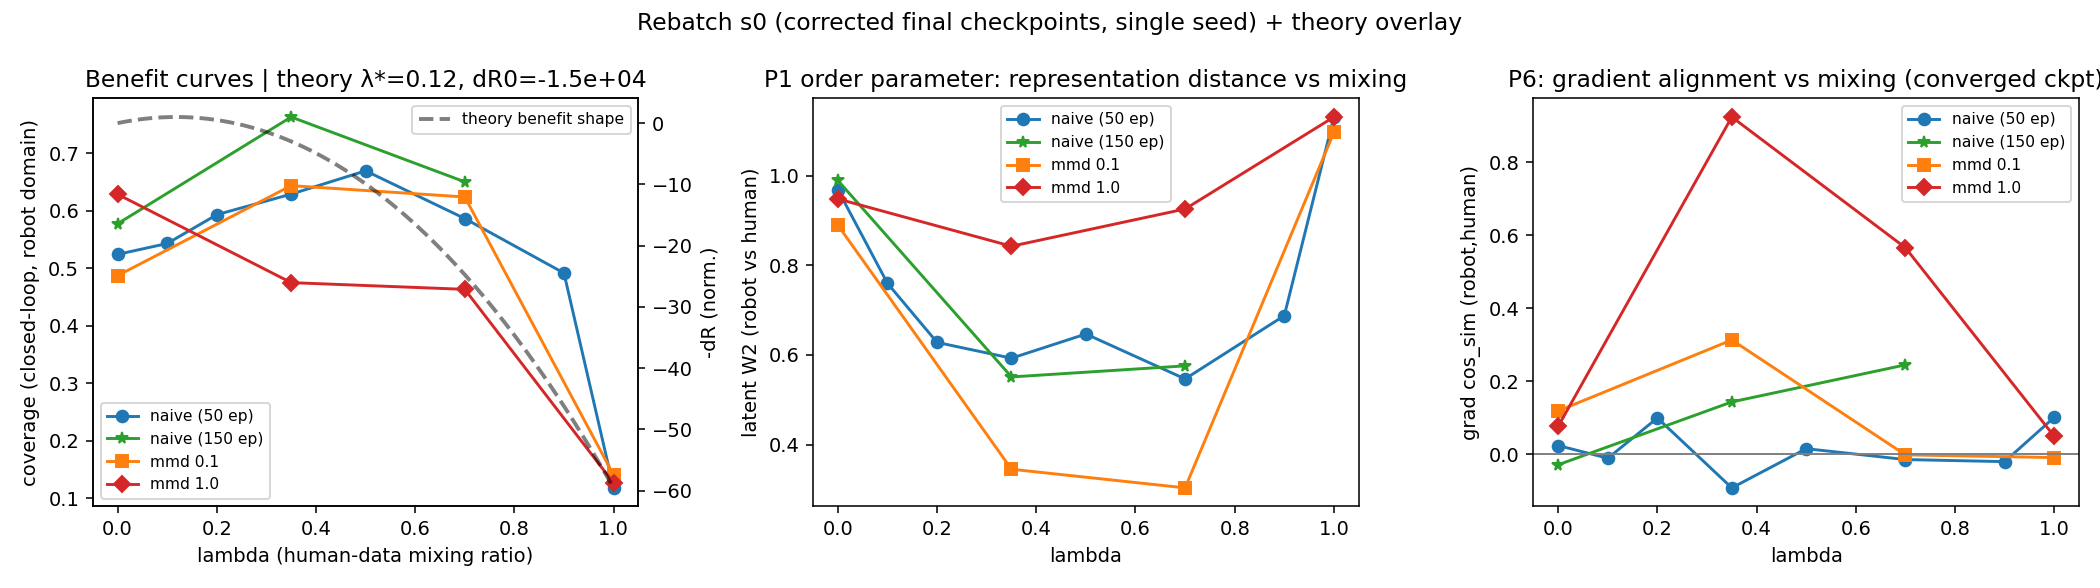
\includegraphics[width=\linewidth]{fig/first_batch.png}
  \caption{\textbf{First batch vs.\ theory.}
  Left: closed-loop coverage vs.\ mixing ratio for the four arms (naive 50-epoch, naive 150-epoch, two MMD weights), with the theoretical benefit shape (dashed; normalized shape comparison only).
  Center: latent-space inter-domain $W_2$.
  Right: robot/human gradient cosine at the converged checkpoint.}
  \label{fig:firstbatch}
\end{figure}

\paragraph{Findings.}
\textbf{(F1)~Non-monotone benefit with an interior optimum --- P2 confirmed at coarse level.}
Naive mixing improves closed-loop coverage over the pure-robot baseline across $0.1 \le \lambda \le 0.9$, peaking at $\lambda^* \approx 0.5$ ($0.670$ vs.\ $0.524$, $+28\%$ relative), and collapses at $\lambda = 1$ ($0.118$) where no robot data remains --- the harm boundary the theory predicts.
\textbf{(F2)~The benefit is not an under-training artifact --- and it relieves overfitting.}
At 150 epochs all arms improve ($\lambda{=}0$: $0.578$) and the mixing benefit \emph{grows}: $\lambda{=}0.35$ reaches $0.763$ ($+32\%$ over its baseline, binary success rate $0.40$ vs.\ $0.25$), $\lambda{=}0.7$ gives $0.650$.
The training logs show why: at 150 epochs the pure-robot run overfits (train/val loss $0.005$/$0.164$), while mixed runs sit at $0.008$/$0.085$--$0.127$ --- human data acts as a variance-reduction regularizer, the model's term B.
The flat curves one would read off an under-trained budget are an artifact of the training regime, not of the mixing structure.
\textbf{(F3)~Open-loop and closed-loop diverge in opposite directions.}
The open-loop robot-domain validation loss improves monotonically with human data all the way to $\lambda = 0.9$ ($0.072 \to 0.036$), while the closed-loop coverage peaks at $\lambda^* \approx 0.5$ and already declines at $\lambda = 0.9$ ($0.492$); at $\lambda = 1$ both collapse ($0.227$, $0.118$).
Past the closed-loop optimum, extra human data still helps \emph{predict} robot actions but hurts \emph{executing} them --- direct evidence that open-loop risk and closed-loop compounding must be bridged explicitly (in the spirit of~\cite{ross2011reduction}), which our current model does not yet cover.
\textbf{(F4)~Alignment strength itself is non-monotone.}
At $\lambda = 0.7$, light MMD ($\alpha_{\mathrm{mmd}} = 0.1$) improves over naive ($0.624$ vs.\ $0.587$), but strong MMD ($\alpha_{\mathrm{mmd}} = 1.0$) \emph{hurts} at intermediate $\lambda$ ($0.475$/$0.464$ vs.\ naive $0.629$/$0.587$).
This is qualitatively consistent with the model's coverage term C: over-aggressive alignment collapses precisely the spectral breadth through which human data helps --- alignment should be tuned, not maximized.
\textbf{(F5)~Representations track the mixing ratio.}
Latent $W_2$ decreases with $\lambda$ in the interior (naive: $0.97 \to 0.55$--$0.65$) and re-expands at $\lambda = 1$ ($1.13$); the gradient cosine at the converged checkpoint is near zero throughout, with sign noise at extreme $\lambda$ --- the probe records the converged state, so training-time conflict tracking is deferred to the multi-seed batch.
\textbf{(F6)~Probe caveats.}
Domain AUC saturates ($\approx 1.0$) and one checkpoint exhibits an ill-conditioned gradient pair (mmd$_{1.0}$, $\lambda{=}0.35$: cos $0.93$, $\kappa(\hat G) = 2.6$); the next batch uses a capacity-limited probe and training-time gradient logging.

\paragraph{Consistency with theory, stated honestly.}
The theory gets right: the \emph{sign} of the marginal benefit, the \emph{existence of an interior optimum}, and the \emph{harm boundary} at $\lambda \to 1$.
It is quantitatively off on the optimum's position: with the testbed's measured near-zero spectral gap and anti-aligned mismatch, Eq.~\eqref{eq:t1a} predicts a small benefit peaked near $\lambda^* \approx 0.12$, while the measured peak sits at $\lambda^* \approx 0.5$ with a substantial amplitude.
This gap is expected at two levels: the model is a linear-ridge asymptotic object while the learner is a 50-epoch diffusion policy, and the mismatch/alignment estimates $\hat\delta$, $\hat c$ come from a linear state-action proxy that need not track the learned policy's effective mismatch.
Closing this quantitative gap (calibrated $\mu$, learned-feature spectra, multi-seed significance) is the purpose of the next batch; the structural agreement reported here is the scope we claim in this paper.
